\section{Analyse}
\label{ch:analyse}
\subsection{Hvordan måler vi hældning?}
Før vi kunne begynde på at lave en hældningssensor, blev vi nødt til at finde ud af hvilke muligheder, der eksisterer for hældningsmåling. \\
En af mulighederne var at anvende et pendul eller en libelle. Vi startede med at udvikle på en prototype af en libellesensor vist på figur \ref{fig:libelle}.
\begin{figure}[hbpt]
\centering
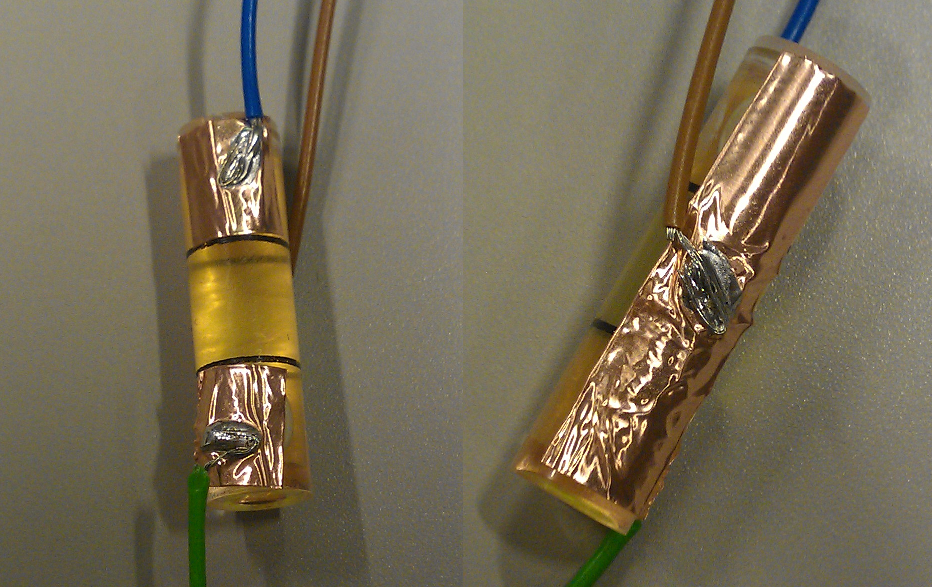
\includegraphics[width=0.4\textwidth]{billeder/libellesensor1}
\caption{Hældningssensor baseret på libelle}
\label{fig:libelle}
\end{figure}
Den første hældningssensorprototype indeholder to højpasfiltrer, en frekvensgenerator og en differensforstærker. Vi kom frem til at libellesensoren har en capacitet på omkring $1*10^{-15}[F]$. Det gør det praktisk talt umuligt at anvende, da vores filter skulle designes til en cutoff frekvens $>3.0[MHz]$. Den høje frekvens giver en stor selvinduktion i vores ledning. Et lavt signal fra hældningssensoren kombineret med stor selvinduktion, gjorde at vi måtte finde en anden løsning.\\
Næste prototype bestod af et potmeter og et pendul. Dog havde potmeteret en for stor friktionsmodstand, der gjorde det for upræcist i forhold til vores krav.\\
Vi har gennem et tredje semestersfag fundet ud af at PSoC'en indeholder et accelerometer\footnote{Se bilag/datablade/KXSC7-2050}. Efter en prototypeopbygning fandt vi ud af at accelerometeret opfyldte de krav, der er stillet i kravspecifikation. \\
Softwaren er implementeret således, at der kan kalibreres for det offset, der er individuelt for hver PSoC.
%%%%%%%%%%%%%%%%%%%%
%%% VBTE %%%%%%%
%%%%%%%%%%%%%%%%%%%%
\subsubsection{Hvordan måler vi niveauet i vandballasttankene?}
Da ingen i projektgruppen havde arbejdet med ultralyd før valgte vi for udfordringens skyld at forsøge med det. Man kunne have valgt at købe en færdiglavet enhed, men det blev vurderet at dette ikke gav ret meget faglig erfaring. Elektroniklaboratoriet lå inde med nogle rå tranducere og receivere, og gruppen ville derfor forsøge at udvikle en afstandsmåler baseret på ultralyd.\\ 
Der blev i starten lavet en del teknologiundersøgelse af ultralyd og tranducere og receivere blev testede for at se hvordan de aggerede. Vi fandt at der var en del destruktive reflektioner. En løsning var at fylde akustisk skum i toppen af tankene, men da det skum der blev anskaffet var elektrisk ledende kunne det ikke anvendes. Herudover blev der lavet forsøg med forskellige ultralydskredse fundet på Internettet, hvilket gav anledning til erfaring og viden. \\
Den valgte metode anvender bursts og kan ses på figur \ref{fig:bursts}. Der er valgt et burst på 250$\mu$s.\\
\begin{figure}[H]
\centering
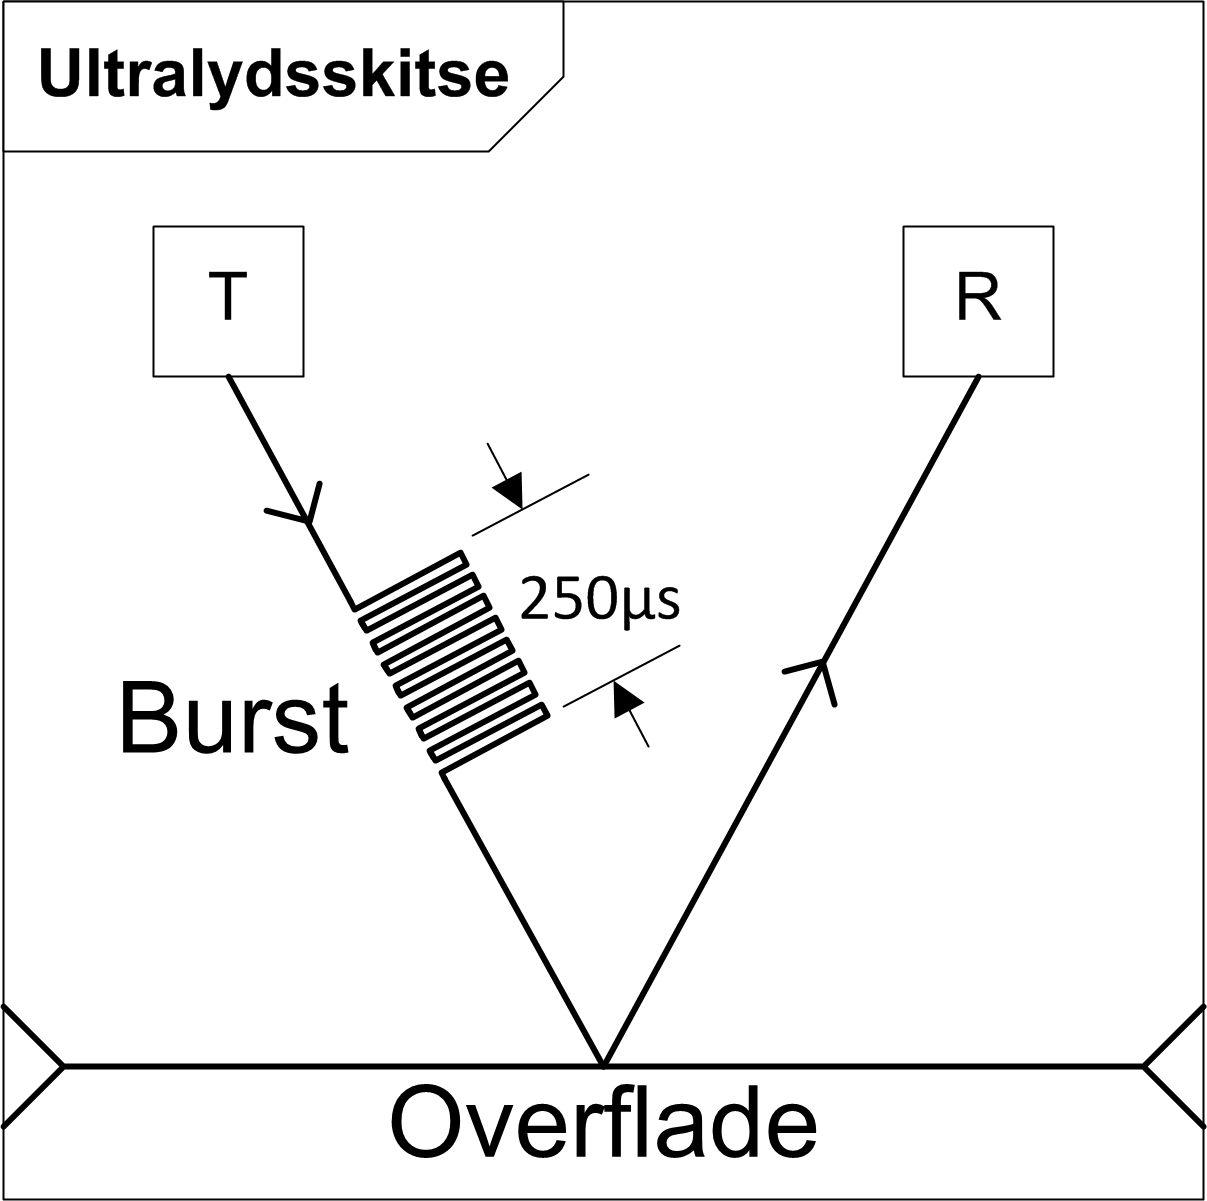
\includegraphics[width=.3\textwidth]{billeder/ultralydsburst}
\caption{illustration af et burst til afstandsmåling}
\label{fig:bursts}
\end{figure}

%%%%%%%%%%%%%%%%%%%%
%%% forsyning %%%%%%
%%%%%%%%%%%%%%%%%%%%
\subsection{Hvordan skal de forskellige modulerne forsynes?}
Da modulerne for eksemplevis kan være placeret ved styrbord, bagbord og midten af skibet, skal der overvejes hvordan de kan forsynes og derigennem overvejes hvilke muligheder der er for forsyningen.
En tanke var om man kunne bruge et batteri eller om der skulle bruges en kablet forsyning:\\\\
\begin{itemize}
\item Batteri:
	\begin{itemize}
	\item Smart, da man undgår at trække en forsyningsledning.
	\item Det kan være meget problematisk med et batteri, da der ikke vides hvor meget strøm der skal trækkes dvs. hvor stort det skal være både i kapicitet og fysisk størrelse. \\
	\end{itemize}
\item Kablet forsyning \\
\begin{itemize}
\item Da der i forvejen er en kablet kommunikation, skal der alligevel kabel ud til modulet.\\
\end{itemize}
\end{itemize}
Ud fra de overstående overvejelser og tanker vil der arbejdes videre med kablet forsyning.
Valget giver anledning til yderligere spørgsmål, for eksempel hvilken forsyningsspænding skal der være?\\
Da forsyningsspændingen på et skib (fx 480V) ligger langt over det der bruges i vores system, skal der bruges en transformator, der kan regulere spænding ned på 24V AC. De 24V AC kan føres ud til modulerne sammen med kommunikationen. \\
Ved modulerne kan der bygges en strømforsyning, der regulerer de 24V AC om til DC. \\
Her kommer der to mulige strømforsyninger op:
\begin{itemize}
\item En SwitchModePowerSupply: \textit{Effektiv, høj virkningsgrad.}
\item En lineær strømforsyning: \textit{Stabil, mellem virkningsgrad}
\end{itemize}
Da virkningsgraden ikke har afgørende betydning for systemet, samt erfaringen med SMPS ikke er stor, vil der tages udgangspunkt i en lineær stømforsyning.\\
Ved udviklingen af prototypen, kan der overvejes om der skal designes en eller flere strømforsyninger.


%%%%%%%%%%%%%%%%%%%%
%%Kontrolinterface%%
%%%%%%%%%%%%%%%%%%%%

\subsection{Raspberry Pi som host for Kontrolinterfacet}
I den indledende fase var det gruppens ønske at kunne implementere Kontrolinterfacet på et Raspberry Pi-modul. Denne mulighed blev undersøgt, og det viste sig at det godt kunne lade sig gøre. Ved at anvende den nyeste beta-version af Qt kunne der skrives programmer til Raspberry Pi'en.\\
Versionerne imellem var der dog store forskelle på fundamentale områder af frameworket; nogle af teknologiundersøgelserne måtte derfor foretages igen.\\
Det var også oprindeligt gruppens ønske at anvende I2C-protokollen mellem Kontrolinterfacet og Styringsmodulet. Denne protokol er også understøttet af Raspberry Pi, men kan kun implementeres med Python medmindre der selv udvikles headerfiler.\\
Dette var en større opgave end gruppen ønskede at prioritere den. Vi begyndte derfor at kigge efter andre protokoller.\\
Næste emne var rs232-protokollen, da den er kendt for gruppen. Protokollen viste sig at være god med Raspberry Pi. Efter nogle teknologiundersøgelser fandt gruppen også ud af hvordan rs232-kommunikationen kunne implementeres med den nye Qt-version.\\
Gruppen løb desvæære igen i problemer, da der skulle kompiles til modulet. Her valgte gruppen at nedprioritere ønsket om at implementere Kontrolinterfacet på Raspberry Pi-modulet og dermed stoppede undersøgelserne.

%%%%%%%%%%%%%%%%%%%%
%%% Databasen %%%%%%
%%%%%%%%%%%%%%%%%%%%
\subsection{Server}
Opbygningen af serveren er gjort på baggrund af behovet for at kunne overføre data via et netværk. Til denne overførelse er TCP blevet valgt grundet erfaring med denne. Ved at benytte TCP kan der være flere end en der kobler til samtidig. TCP giver stabilitet og sikker dataoverførelse. Dette er prioriteret højt i prototypen, da systemet skal være sikkert under lastning og losning. Sikker dataoverførelse sikrer at hvis en pakke går tabt under overførelsen vil denne automatisk blive forsøgt sendt igen. Data vil således også komme frem i korrekt rækkefølge.\\
Fra starten var det meningen at Serveren skulle gemme data direkte til MySQL-databasen, men grundet problemer med at kompile MySQL-header og -driver blev dette efter noget tid droppet. I stedet blev backup-muligheden, der også er indskrevet i kravspecifikationen, fremtaget som eneste mulighed.

\subsection{Valg af database}
For at vælge database til systemet blev der kigge på MySQL, Microsoft Acces og en lagring til en tekstfil.\\
At lagre direkte i en tekst fil blev overvejet, da det er meget simpelt at lagre til tekstfiler fra c++ og php kan håndtere at hente fra den. Det kan gå galt ved loading og lagring til filen samtidig med at formater kan blive et problem. \\
Der var i forvejen kendskab til MySQL og dette er et færdigudviklet system, der fungerer med webinterfaces og for programmeringssprog som C++ er der udviklet headere. Systemet er et system der fungere på mange platforme og løbende bliver udviklet på. På baggrund af dette blev dette system valgt.

\subsection{Webinterface}
Til den grafiske brugergrænseflade for Databasen blev et webinterface valgt for at flere på havneterminalen kunne tilgå data på samme tid. På baggrund af et middel kendskab til interpretere sproget php og dens integration med MySQL-databaser blev php valgt. Php giver desuden mulighed for at benytte ajax princippet og at bygge en hovedside der inkluderer de andre sider. I sidste ende vil dette valg give simplere vedligholdelsen og mindske overførelsestiden til slutbrugeren.\\
Websitet er implementeret på en Apacheserver. Apacheserveren gør det muligt senere at højne sikkerheden på websitet.

%%%%%%%%%%%%%%%%%%%%
%%% Jura %%%%%%
%%%%%%%%%%%%%%%%%%%%
\subsection{Jura}
I startfasen blev de forskellige juridiske problemstillinger undersøgt. Dette gav grund til en del overvejelser omkring opbygningen af systemet BROS. Ansvarshavende personer samt krav til ballastvand er blevet overvejet. Et udpluk af de vigtigste begreber findes i \textit{bilag for Jura}.
For at få en uddybning af disse problemstillinger er Maersk A/S blevet kontaktet. Desværre har vi ikke fået noget svar. De juridske problemstillinger har blandt andet gjort at projektet blev indskrænket til kun at omhandle bulkskibe i nationalt farvand.

